% !TEX encoding = UTF-8 Unicode
%!TEX root = thesis.tex
% !TEX spellcheck = en-US
%%=========================================
\addcontentsline{toc}{section}{Preface}
\section*{Preface}


% Something, something...

With this research my time as at NTNU comes to an end. Six years of studies, and more prominently, being a student, has left me inspired and hungry to employ my knowledge to solve real world problems. As such, the thesis before you describes one real world problem and my attempt at solving it.

For this opportunity, I would like to thank my supervisors Ekaterina Prasolova-Førland and Gabriel Kiss, allowing me to pursuit such practical research has been most rewarding. Without fail, Prasolova-Førland has been indispensable both through resources, organizing and her steady support. 
A huge thanks also to Menno P. Witter at the Kavli Institute for bringing forth this problem, for his incredible knowledge of neuroanatomy and most of all for his positivity and humor, every interaction with Witter has been a joy. 
% I would also like to thank all test participants
% When reflecting on the years of studenthood 

During my years as a student I have had the pleasure to meet many new people, two of which have meant much to me and this resulting thesis. First, my girlfriend, Mathilde Theisen, we found each other during a student trip and have during our studies shared an interest for both technology and outdoor activity. And my friend Ask Jentoft, who I met during a summer project where we created our first application using AR technology, and who has sat besides me writing his own master's thesis on medical use of this technology. Many thanks to you both for your help and support, this project would not be complete without you.\\[2cm]


\begin{center}
Trondheim, 24. June 2021 \\[1pc]
\begin{figure}[H]
    \centering
    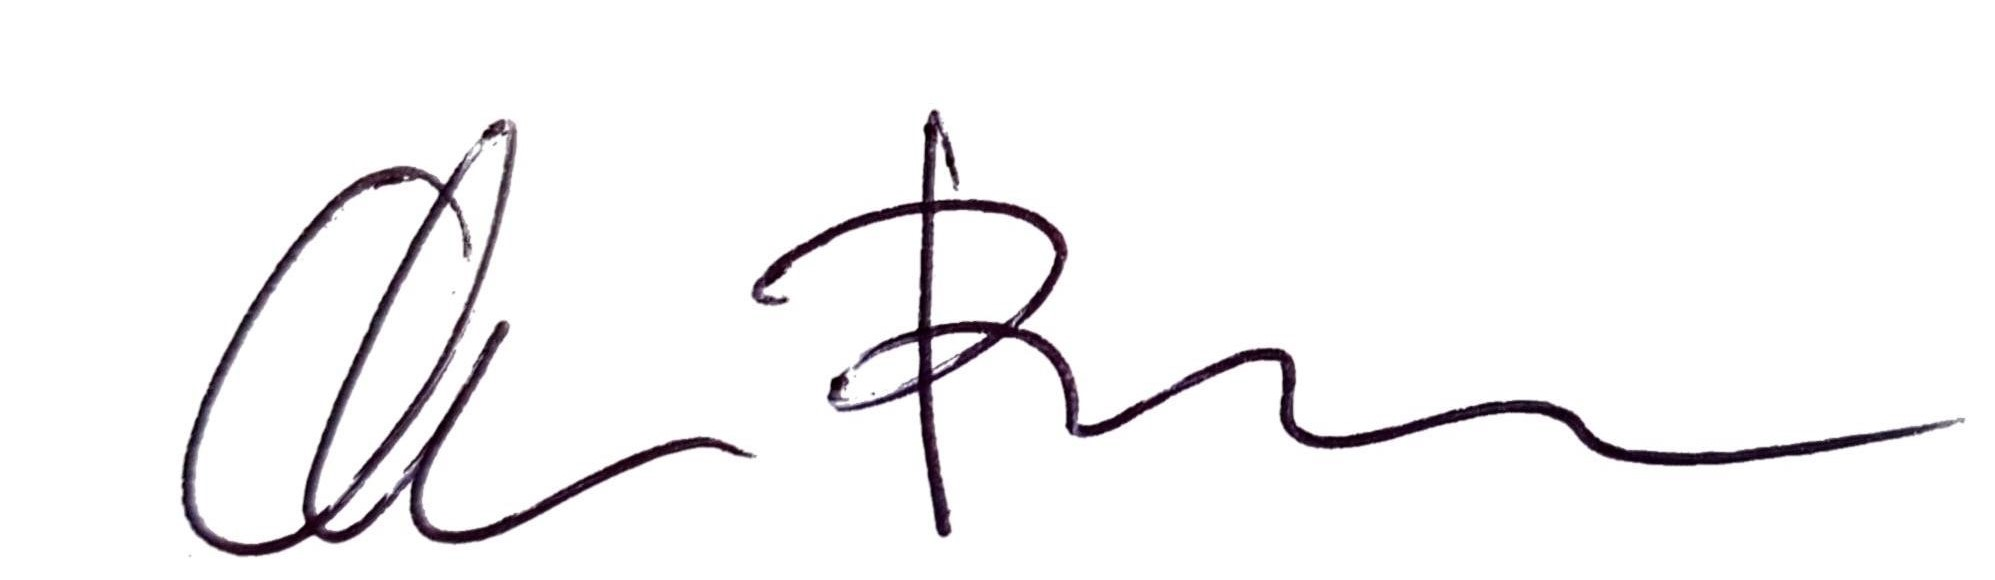
\includegraphics[width=0.3\textwidth , trim={0 0 0 0}, clip]{fig/ravnasign}
\end{figure}
% (Your signature)\\[1pc]
Ole Ravna
\end{center}